\chapter{8. Composite Pattern}
\section{Giới thiệu tổng quan}

Nhắc đến cụm từ \textbf{Composite} thì \textbf{Composite} được hiểu như một thứ được tạo nên từ các thành phần. Một \textbf{Đối tượng Composite} là một đối tượng được tạo nên bởi nhiều đối tượng. Ví dụ như một chiếc ô tô được tạo nên bởi 4 chiếc bánh xe vậy hay nước được tạo bởi Hydro và Oxy vậy. Đó là cách mà \textbf{Composite Pattern} được tạo ra. Xét những trường hợp mà ta muốn gom một nhóm đối tượng thành một tập hợp để thuận tiện trong quá trình thao tác

\section{Định nghĩa và Mô hình cấu trúc}
\subsection{Định nghĩa}
\textbf{Composite Pattern} cho phép ta tổ chức những đối tượng dưới dạng cây phân tầng. \textbf{Composite} cho phép coi các đối tượng riêng lẻ và các thành phần của các đối tượng như một thể thống nhất

\begin{figure}[!htb]
    \centering
    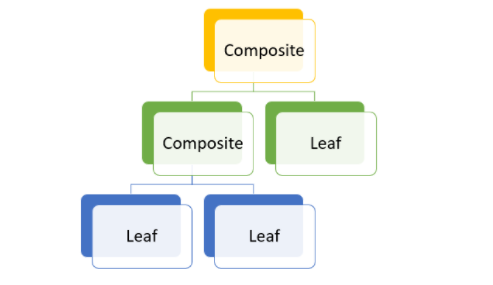
\includegraphics[width=\textwidth]{fig/Composite/CompositeStructure.png}/
\end{figure}
\newpage
\subsection{Mô hình cấu trúc}
Mô hình cấu trúc của \textbf{Composite Pattern} được biểu diễn như sau:

\begin{figure}[!htb]
    \centering
    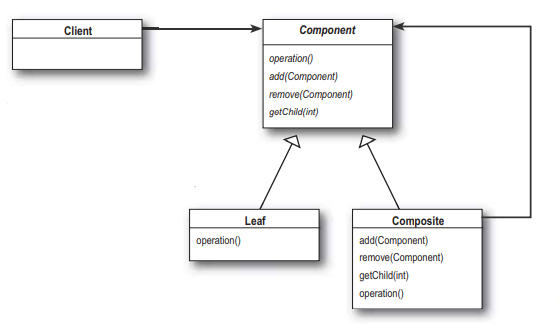
\includegraphics[width=\textwidth]{fig/Composite/CompositeDiagram.png}/
\end{figure}

\begin{itemize}
    \item \textbf{Base Component}: Là một \textbf{Interface} hoặc \textbf{Abstract Class} quy định các phương thức chung cần phải có cho tất cả các thành phần tham gia
    \item \textbf{Leaf}: Là lớp thực hiện cài đặt phương thức của \textbf{Component} và không chứa lớp con
    \item \textbf{Composite}: Là lớp có vai trò lưu trữ và thao tác tập hợp các \textbf{Leaf}
    \item \textbf{Client}: Là nơi sử dụng \textbf{Base Component} để làm việc với các đối tượng trong \textbf{Composition}
\end{itemize}\smallskip

\textbf{Lưu ý}: Một \textbf{composite} chứa các \textbf{component} vì \textbf{component} có thể là \textbf{composite} hoặc \textbf{leaf}. Nghe vẻ có mùi đệ quy ở đây nhỉ? Có vẻ là vậy vì một \textbf{composite} chứa tập hợp các nút con, những nút con có thể là \textbf{composite} hoặc \textbf{leaf}\newpage

\section{Ví dụ}

Để hiểu hơn Composite Pattern, xét ví dụ về bài toán quản lý tệp tin:

\begin{figure}[!htb]
    \centering
    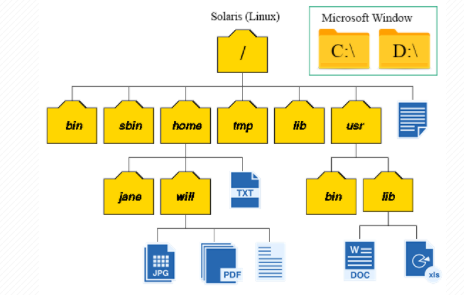
\includegraphics[width=\textwidth]{fig/Composite/FileStructure.png}/
\end{figure}

Một hệ thống tệp tin là hệ thống có cấu trúc cây phân cấp trong đó có các File và Folder. Một Folder có thể chứa nhiều File và Folder bên trong nên ta có thể coi Folder như \textbf{Composite} còn File sẽ là \textbf{Leaf}. Ta có mô hình cấu trúc ở bên dưới:

\begin{figure}[!htb]
    \centering
    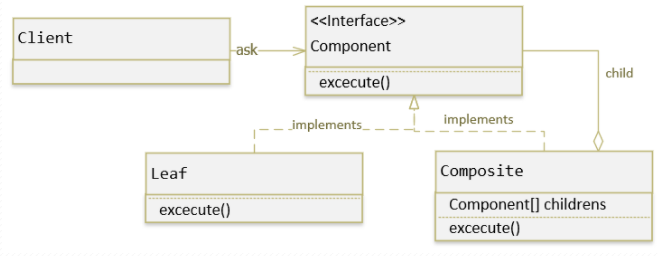
\includegraphics[width=\textwidth]{fig/Composite/FileDiagram.png}/
\end{figure}\newpage

Đầu tiên ta định nghĩa cho \textbf{component} Interface có các phương thức chung cho cả File và Folder. Để đơn giản, ví dụ này chỉ bảo gồm 2 phương thức \textbf{showProperty()} và \textbf{totalSize()}. Hai phương thức này sẽ lấy ra thông tin của File/Folder và tổng kích thước của chúng

\begin{figure}[!htb]
    \centering
    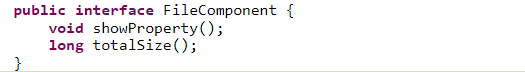
\includegraphics[width=\textwidth]{fig/Composite/FileComponent.png}/
\end{figure}

Tiếp theo, ta tạo lớp \textbf{Leaf} cài đặt các phương thức của \textbf{component}, gọi là \textbf{FileLeaf}. Sau đó tạo lớp \textbf{Composite} chứa tập hợp các \textbf{Leaf} và cài đặt các phương thức của lớp \textbf{component}, gọi là \textbf{FolderComposite}\\[0.1in]

Lớp \textbf{FileLeaf}:
\begin{figure}[!htb]
    \centering
    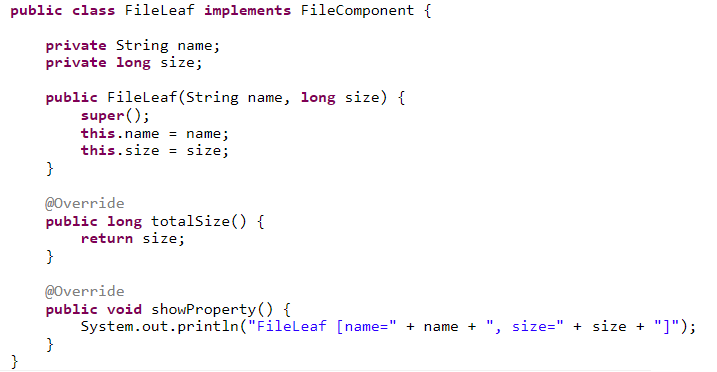
\includegraphics[width=\textwidth]{fig/Composite/FileLeaf.png}/
\end{figure}\newpage

Lớp \textbf{FolderComposite}:
\begin{figure}[!htb]
    \centering
    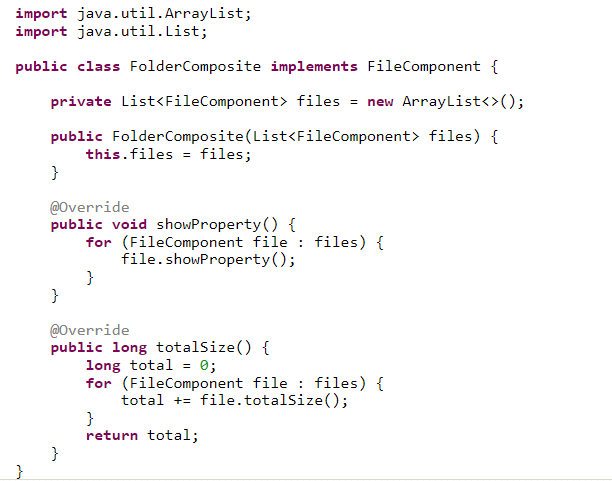
\includegraphics[width=\textwidth]{fig/Composite/FolderComposite.png}/
\end{figure}

Cuối cùng, ta hoàn thiện lớp \textbf{Client} để chạy chương trình:
\begin{figure}[!htb]
    \centering
    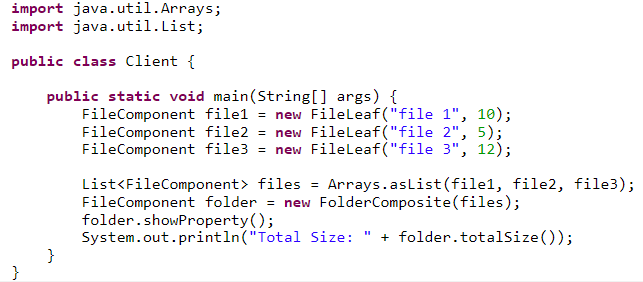
\includegraphics[width=\textwidth]{fig/Composite/FileClient.png}/
\end{figure}\newpage

Output của chương trình:
\begin{figure}[!htb]
    \centering
    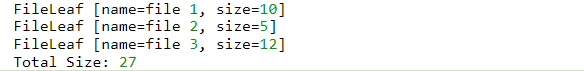
\includegraphics[width=\textwidth]{fig/Composite/FileOutput.png}/
\end{figure}

\section{Thực tế}
\textbf{Composite Pattern} có thể được tìm thấy tại hầu hết các hệ thống lập trình theo hướng đối tượng. Lớp Viewer gốc của Smalltalk Model/View/Controller [KP88] là \textbf{Composite}, và gần như bộ giao diện người dùng và framework. Viewer thời điểm đó vừa là lớp \textbf{Component} vừa là lớp \textbf{Composite}. Bản 4.0 của Smalltalk-80 sửa lại Model/View/Controller với một lớp VisualComponent có những lớp con là View và CompositeView\\[0.1in]
RTL Smalltalk compiler framework sử dụng Composite Pattern một cách chuyên sâu. RTLExpression là một lớp \textbf{Component} cho cây phân tích cú pháp. Nó có những lớp con như BinaryExpression chứa những đối tượng RTLExpression. Những lớp này định nghĩa một cấu trúc composite cho cây phân tích cú pháp. RegisterTransfer là một lớp \textbf{Component} cho chương trình trung gian Single Static Assignment (SSA). Những lớp con Leaf của RegisterTransfer xác định các nhiệm vụ tĩnh khác nhau\\[0.1in]
Một ví dụ khác cho pattern này xảy ra trong lĩnh vực tài chính, nơi mà có một danh mục đầu tư tổng hợp các tài sản riêng lẻ. 
Ta có thể hỗ trợ các tổng hợp phức tạp của tài sản bằng cách cài đặt "danh mục đầu tư" như một lớp \textbf{Composite} phù hợp với giao diện của một tài sản cá nhân [BE93].